\section{Rakenne} \label{rakenne}
Seuraavaksi esitellään reunajärjestelmän rakennetta.
Koska aihepiirinä on arkkitehtuurit, varsinaisten toteutettavien reunajärjestelmien rakennetta voidaan tarkastella ainoastaan implisiittisesti. 
Eli mitä arkkitehtuurit mahdollistavat tai rajoittavat.
Ensimmäiseksi esitellään reunan fyysisen rakenteen eri mallit, jossa keskeisessä osassa ovat reunasolmujen sijainnit.
Tämän jälkeen käsitellään reuna-arkkitehtuurien vaikutuksen toteutettavaan järjestelmään.

Erilaiset rakenteet voidaan jakaa kahteen päätyyppiin: litteään ja hierarkkiseen.
Litteä rakenne edustaa yksinkertaisempaa lähestymistapaa resurssien asetteluun. Hierarkkinen rakenne puolestaan edustaa hallinnollisesti monimutkaisempaa järjestelmää, jossa reunasolmut voivat delegoivat tehtäviä suhteessa tehokkaammille ja keskitetymmille reunasolmuille. 

Reunan rakenteeseen vaikuttaa myös tapa jolla järjestelmä tuotetaan.
Esimerkiksi tilanne jossa reunajärjestelmä toteutetaan siten, että yksityisen toimijat, kuten yritykset, voivat hankkia omia reunasolmuja ja liittää niitä osaksi reunajärjestelmää. Tällöin reunajärjestelmän rakenne on vaihteleva eikä siihen todennäköisesti litteä.
Tällaisessa tilanteessa keskeiseksi tekijäksi nouseekin reunapalveluiden tuottamiseen käytettävä liiketoimintamalli.
Yksinkertaisuuden vuoksi tässä kappaleessa aihetta käsitellään, kuin reunan rakenne olisi yhden entiteetin, esimerkiksi operaattorin, päätettävissä. 

\paragraph*{Reunavyöhyke}
Reunavyöhyke on tämän tutkielman puitteissa määritelty termi, jolla viitataan vyöhykkeeseen, jolla reunasolmut sijaitsevat. Reunavyöhyke voi olla kapea tai leveä, jotka vastaavat suurin piirtein seuraavaksi määriteltävää litteää ja hierarkkista rakennetta. Kapea vyöhyke tarkoittaa että reunasolmut sijaitsevat verkossa samalla tasolla. Leveä vyöhyke puolestaan viittaa rakenteeseen jossa reunasolmujen etäisyys asiakkaasta vaihtelee merkittävästi. Leveässä järjestelmässä reunasolmut voivat sijaita esimerkiksi lähimmillään tukiasemassa ja kauimmillaan mobiiliverkon ulkopuolella sijaitsevassa palvelinsalissa. 

\begin{figure}[tb]
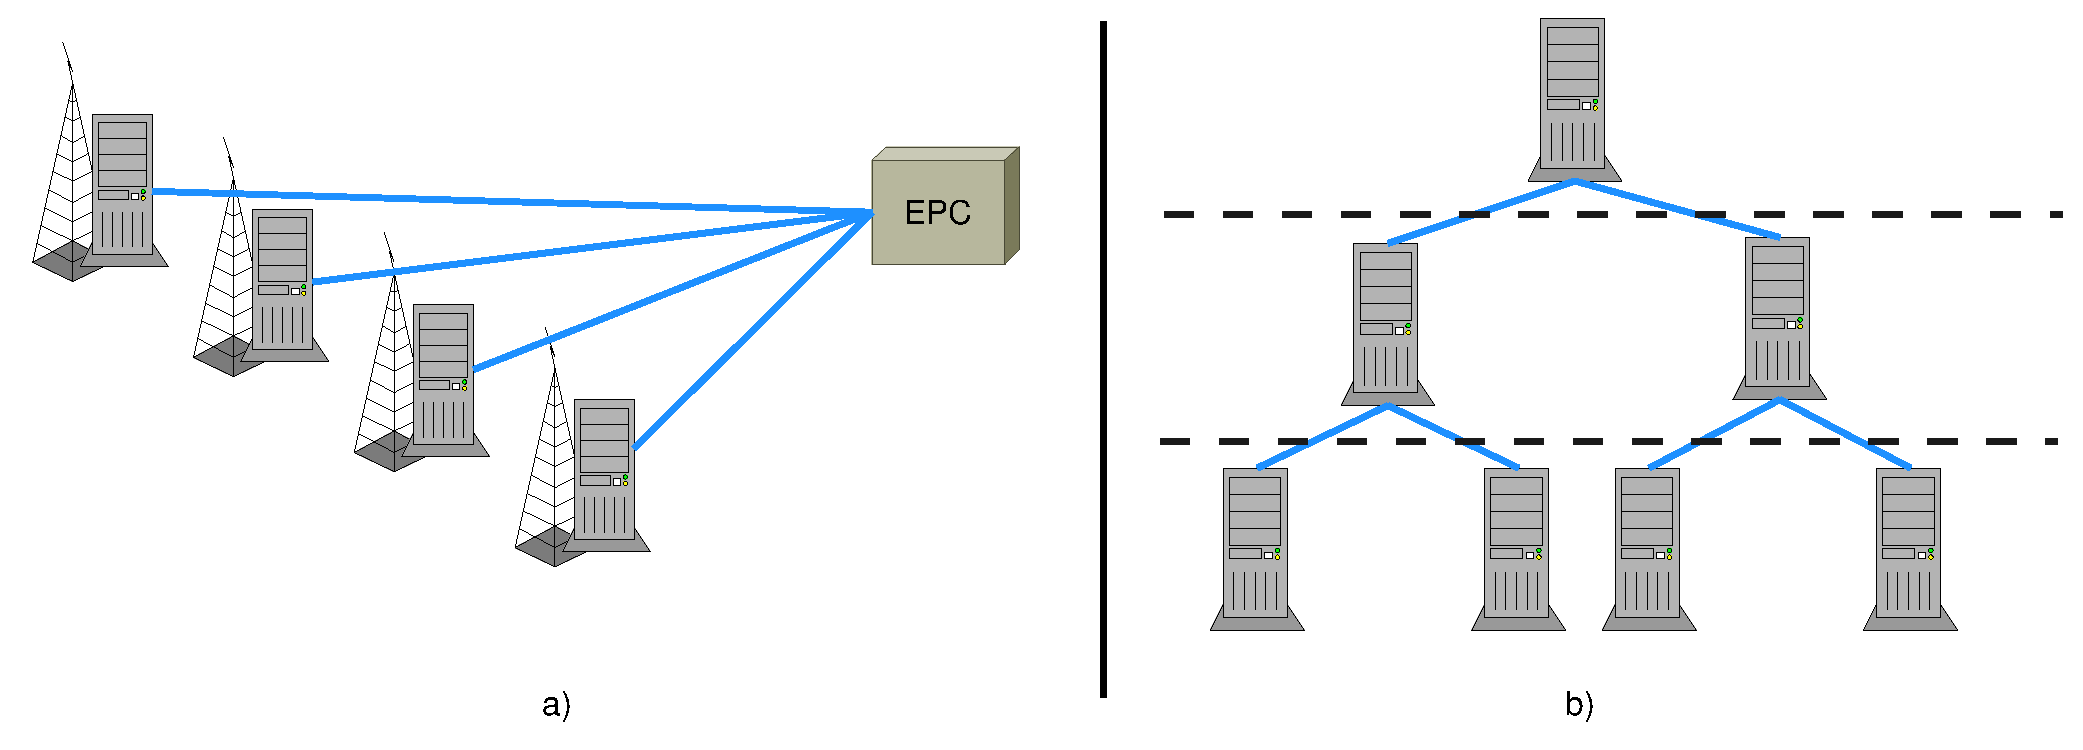
\includegraphics[width = \textwidth]{rakenne.eps}
\caption{Esimerkki rakenteet a) litteä rakenne b) hierarkkinen rakenne kolmella tasolla} \label{fig:rakenne}
\end{figure}

\subsubsection{Litteä rakenne}
Litteällä rakenteella tarkoitetaan että reunasolmut sijaitsevat vain yhdessä kerroksessa. Litteän järjestelmän keskeisin päätös on valita taso, jolle reunasolmut sijoitetaan.

Yksinkertainen esimerkki litteästä toteutuksesta olisi reunajärjestelmä, jossa reunasolmut sijoitettaisiin mobiiliverkon tukiasemien yhteyteen kuten kuvassa \ref{fig:rakenne} a). Tämän kuvan esimerkin järjestelmä  toteuttaisi äärimmäistä hajautusta. Se olisi fyysisesti erittäin lähellä asiakaslaitetta ja näin ollen pystyisi teoriassa tarjoamaan palvelua kaikkein pienimmällä viiveellä \cite{mach17mobile}.
Vaikka viiveet olisivat pienet, on tällaisessa ratkaisussa ongelmia.
Järjestelmän käyttö olisi teoriassa mahdollista ainoastaan niiden tukiasemien ympäristössä, joissa reunajärjestelmä sijaitsee. Tämän seurauksena reunalaskennan laajamittainen käyttöönotto olisi riippuvainen tukiasemiin sijoitettavien reunasolmujen hankinnasta. Kun otetaan huomioon trendi, jossa mobiiliverkon solut pienevät, niin ainoastaan tukiasemiin sijoitettavien reunasolmujen käyttöönotto vaikuttaa epärealistiselta skenaariolta.

Mikäli oletetaan, että siellä missä laskennan tarve on suurin, on myös eniten ihmisiä. Yleensä tällaisissa sijainneissa myös reunajärjestelmän resursseja varten tarvittavien tilojen hinnat ovat korkeammat, jolloin reunalaskennan tuominen lähelle asiakasta nostaa reunajärjestelmän hintaa \cite{mao17}.
Vaihtoehtoinen ratkaisu olisi siirtää reunasolmuja kauemmaksi tukiasemista. Esimerkiksi siten, että yksi reunasolmu vastaisikin useamman tukiaseman kautta tulevasta reunalaskennasta.
Mobiiliverkko kontekstissa, reunasolmu sijaitsisi siis joko tukiasemien ja EPC:n välillä tai vasta EPC:n takana.  
Useamman tukiaseman niputtamista yhden reunasolmun vastuulle kutsutaan klusteroinniksi \cite{RefWorks:doc:59d4b224e4b015703b881ab9}. 
Keskeisenä haasteena klusteroinnissa on valita oikean kokoiset klusterit ja sijoittaa oikea määrä resursseja kuhunkin klusteriin \cite{malandrino2016close}.
Klusterin suuruus ja viive todennäköisesti korreloivat, jolloin on varottava tekemästä klustereista tarpeettoman suuria.
Klusteroinnin pitäisi kuitenkin mahdollistaa helpompi ja edullisempi käyttöönotto, koska tarvitaan suhteessa vähemmän reunasolmuja ja reunasolmujen ylläpito on näin ollen edullisempaa.
Kompromissina on kuitenkin suurempi viive reunasolmujen ja asiakaslaitteiden välillä. 
Onkin siis tärkeää että reunasolmuja ei viedä liian kauas reunasta, jottei palvelun laatu heikkene \cite{mao17}. 


Kuitenkin riippumatta litteän rakenteen sijainnista, sen pohjimmaisena ongelmana on resurssien kohdistuminen jollekkin tietylle palvelualueelle. Ympäristössä jossa reunalaskennan määrä vaihtelee, seuraa tilanne jossa reunasolmu on joko ylikuormitettuna tai alikuormitettuna suhteessa käytössä oleviin resursseihin \cite{tong2016hierarchical}. Jotta reunasolmut pystyisivät suoriutumaan kaikesta reunalaskennasta, reunasolmujen resurssit jouduttaisiin mitoittamaan rasitushuippujen mukaan. Tästä seuraa lähes jatkuvaa alikuormitusta, joka tarkoittaa että reunajärjestelmän kustannukset kasvavat resurssihankintojen seurauksena. 
Tämän ongelman ratkaisuksi on esitetty hierarkkista järjestelmää.


%In 2012, Flavio Bonomi and his colleagues introduced the term fog computing to refer to this dispersed cloud infrastructure. F. Bonomi et al., “Fog Computing and Its Role in the Internet of Things,”Proc. 1st Edition MCC Workshop Mobile Cloud Computing (MCC 12)


\subsubsection{Hierarkkinen rakenne}
Hierarkkinen rakenne on parannusehdotus reunalaskennan oletetulle litteälle rakenteelle \cite{tong2016hierarchical}.
Reunasolmujen hierarkkisella asettelulla tarkoitetaan järjestelmää, jossa reunasolmut on jaettu kerroksiin. Alimmalla kerroksella sijaitsevat reunasolmut ovat lähimpänä asiakaslaitetta, mutta niiden sisältämät laskentaresurssit ovat vähäisiä. 
Ideana on että alemmalla kerroksessa sijaitsevat reunasolmut voivat siirtää laskentaa ylemmällä kerroksella sijaitsevalle reunasolmulle, jolla on enemmän resursseja. Tasojen määrälle ei ole mitään rajaa, mutta useimmat ehdotukset sisältävät kaksi tai kolme tasoa. Kuvassa \ref{fig:rakenne} b) esimerkki kolmetasoisesta hierarkiasta.
Ylemmällä tasolla sijaitsevalla reunasolmulla on vastuullaan useampi alemman tason reunasolmu. Hierarkkinen rakenne on siis puun mallinen.

Hierarkkisen rakenteen keskeisenä tavoitteena on reunajärjestelmän resurssien käyttöasteen parantaminen \cite{tong2016hierarchical}. Ylemmillä kerroksilla sijaitsevat resurssit ovat suuremman joukon käytössä, hieman kuten litteässä mallissa tukiasemia klusteroitaessa. 
Hierarkkisessa rakenteessa on kuitenkin riskinsä. Järjestelmän voidaan olettaa monimutkaistuvan jos laskentaa tehdään useassa kerroksessa. Ja etenkin järjestelmän ylempien kerroksien etäisyys asiakaslaitteisiin kasvaa, joka voi potentiaalisesti johtaa viiveiden kasvuun ja palvelun laadun heikkenemiseen.

Tong et al. esittävät tutkimuksessaan vertailua litteälle ja erilaisille hierarkkisille rakenteille \cite{tong2016hierarchical}. Tilanteessa jossa järjestelmään on jaettavissa kiinteä määrä resursseja, kolmeen kerrokseen jaettu järjestelmä vaikutti optimaalisimmalta.
Vertailun mittarina käytettiin aikaa joka reunapalvelulla kului vastata annettuihin laskennallisiin tehtäviin. Kolmikerroksisen mallin etuina oli laskentaresurssien määrä ylemmillä kerroksilla. Tällöin etenkin ruuhkaisissa tilanteissa se suoriutui tehtävistään nopeammin kuin litteä. Lisäksi tutkimuksessa todettiin, että ylemmillä tasoilla sijaitseva tehokkaampi laskenta pystyy kompensoimaan siirtämisestä aiheutuvaa viivettä. Huomattakoon kuitenkin että tutkimuksessa käytettävä kuorma oli tyypiltään hienojakoista ja pientä. 


\subsubsection{Yhteenveto}
Hierarkkinen järjestelmä on potentiaalinen vaihtoehto litteälle rakenteelle. Koska reunalaskennalle on monia hyvin erilaisia sovelluskohteita, hierarkkinen rakenne vaatii tarkempaa tutkimusta erilaisilla reunalaskennan tyypeillä. Litteän rakenteen heikkoina puolina voidaan pitää sen kyvyttömyyttä sopeutua kuorman epätasaisuuteen, sekä järjestelmän ylläpidon kustannuksia, mikäli järjestelmää päätetään hajauttaa aggressiivisesti. Litteä järjestelmä on rakenteeltaan yksinkertainen ja se tukee esimerkiksi olemassa olevaa mobiiliverkon tukiasemien rakennetta. 


\subsection{Arkkitehtuurin vaikutus}
Edellisessä kappaleessa järjestelmän rakenteen oletettiin olevan vapaa sijoittamaan reunasolmut haluamiinsa paikkoihin. 
Todellisuudessa reuna-arkkitehtuurit kuitenkin asettavat joitakin rajoitteita reunasolmujen sijaintien suhteen. Seuraavaksi käsitellään reuna-arkkitehtuurin vaikutusta reunasolmujen sijoitteluun.

%mobiiliverkko
Tutkielmaan valitut arkkitehtuurit sitovat jo lähtökohtaisesti reunajärjestelmää osaksi mobiiliverkkoa. Integraation tyypillä on tässäkin yhteydessä vaikutus siihen, kuinka paljon reunajärjestelmän rakenne on sidoksissa mobiiliverkkoon.
Tämän lisäksi kommunikaatioväylien toteutus vaikuttaa rakenteeseen. 
Arkkitehtuureissa joiden kommunikaatioväylät eivät nojaa mobiiliverkon sisällä tapahtuvaan reititykseen ovat vapaampia sijoittamaan reunasolmuja. 
Hallinnolliset toimijat ovat, joko mobiiliverkkoon integroituina tai mobiiliverkon ulkopuolella. Hallinnollisien entiteettien sijaintiin vaikuttaa pääasiassa se, onko niillä rajapintaa mobiiliverkon sisäisten toimijoiden kanssa. Mikäli on, niin ne sijaitsevat loogisesti osana mobiiliverkkoa. 
Koska reunasolmujen sijoittuminen on hyvin riippuvaista arkkitehtuuristaehdotuksesta, reunasolmujen sijoittumista käsitellään seuraavassa kappaleessa jokaisen arkkitehtuuriehdotuksen yhteydessä.

Reunanajärjestelmän riippuvuutta mobiiliverkkoon voidaan yrittää pienentää, esimerkiksi ottamalla SDN käyttöön. SDN mahdollistaa tietoliikennevirtojen ohjaamisen siten, että reunajärjestelmän tietoliikennevirrat eivät vaikuta mobiiliverkon toimintaan. Tämän seurauksena reunajärjestelmä on täysin vapaa sijoittamaan reunasolmut haluamiinsa sijainteihi. Keskeinen viiveeseen vaikuttava ratkaisu on SDN verkon sijoittuminen mobiiliverkon hierarkiassa.

Toinen ehdotettu ratkaisu on liittä reunasolmut tukiasemiin. Tämä pakottaa järjestelmälle litteän rakenteen.
Tällainen järjestelmä on siis reunasolmujen osalta sidoksissa mobiiliverkon rakenteeseen. Small Cell Cloud (käsitellään kappaleessa \ref{scc}) esittää tämänkaltaista ratkaisua.
Ideana on että tukiasemien tarjoamat solut ovat pieniä, jolloin tukiaseman kantama olisi pieni ja täten palveltavien asiakaslaitteiden määrä myös vähäinen. Tällöin tukiasemaan tarvittavien reunalaskentaresurssien määrä on myös vähäisempi, verrattuna tilanteeseen jossa tukiasemalla olisi enemmän palveltavia. 

Kolmas ja viimeinen tyyppi on kokonaan mobiiliverkon ulkopuolelle sijoitetut reunasolmut. Tämä antaa käytännössä täydellisen vapauden sijoitella reunasolmuja. Esimerkki tämänkaltaisesta arkkitehtuurista on Follow Me Cloud (käsitellään kappaleessa \ref{fmc}). Reunajärjestelmän sijoittaminen mobiiliverkon ulkopuolelle tarkoittaa, että asiakaslaitteen ja reunasolmun välinen viive on vähintään se aika joka tietoliikenteellä kuluu mobiiliverkossa. Follow Me Cloudin tapauksessa oletetaankin, että mobiiliverkon aiheuttamaa viivettä voitaisiin pienentää ja että reunasolmut sijaitsisivat välittömästi mobiiliverkon ulkopuolella. 

%arkkitehtuurin asettamat rajoitteet
%hallinnon sijainti
%integraatio mobiiliverkkoon
%hallinnoivan järjestelmän omistajuus.

%mobiili














